\chapter{Výběr algoritmu pro detekci pózy}
\label{sec:Pose}

Jelikož je dnes dostupných mnoho různých algoritmů či modelů pro detekci pózy
osob v obrázku či videu, nemá smysl pro naše řešení tvořit takovýto algoritmus
od nuly. Možné by to samozřejmě bylo, i vzhledem k dostupnosti otevřených
trénovacích dat (např. dataset COCO \cite{coco}), nicméně bychom pravděpodobně
nedosáhli kvalitních výsledků, jako řešení, která jsou výsledkem mnoholetých
výzkumů. Hlavně pak bychom těžko dosáhli výkonů těchto řešení, a ten je pro nás
stěžejní, jelikož potřebujeme video zpracovávat v reálném čase.

V následující kapitole budou popsány obecné principy detekce osob a jejich pózy
v obraze. Následně budou popsány některé populární algoritmy pro detekci pózy
se zaměřením na jejich specifika. Několik z nich pak bude otestováno, výsledky
budou porovnány, a na jejich základě bude zvolen algoritmus použitý v konečném
řešení detekce pádu.

\section{Detekce pózy}

\begin{figure}[]
    \centering
    \begin{minipage}{0.48\textwidth}
        \centering
        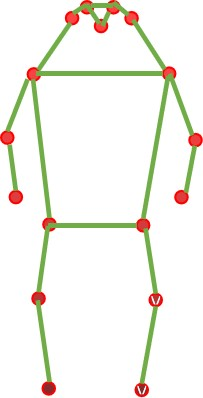
\includegraphics[width=0.5\textwidth]{Figures/keypoints.png}
    \end{minipage}
    \hfill
    \begin{minipage}{0.48\textwidth}
        \centering
        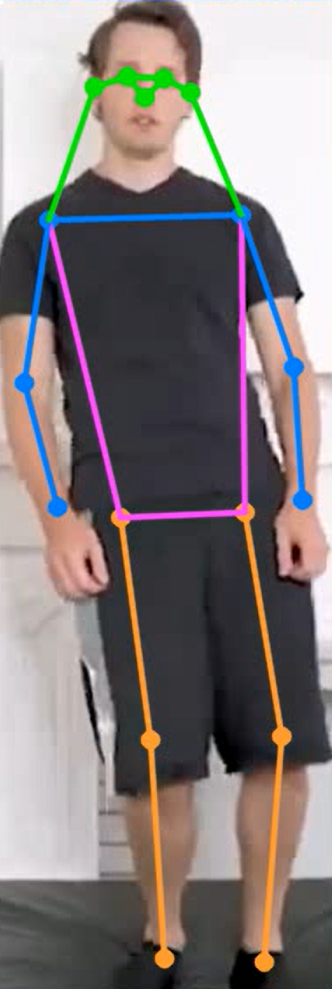
\includegraphics[width=0.35\textwidth]{Figures/pose1.png}
    \end{minipage}
    \caption{(Vlevo) Topologie klíčových bodů použitá např. v COCO-pose.\cite{2dhpe} (Vpravo) Příklad detekce pózy pomocí YOLO.}
    \label{fig:keypoints}
\end{figure}

Uloha detekce pózy spočívá v nalezení klíčových bodů postavy v obraze. Může se
jednat také o zvíře, v našem případě se ale budeme zabývat pouze klíčovými body
lidské postavy. Klíčové body představují důležité body lidského těla, znalost
jejich lokalizace nám umožňuje analyzovat pózu dané osoby, popřípadě sledovat
její pohyb. K základním klíčovým bodům patří hlava, ramena, lokty, zápěstí,
kyčle, kolena a kotníky, viz \ref{fig:keypoints}. Některé algoritmy dokážou
rozeznat i orientaci dlaně či stopy, nebo rozpoznat klíčové body na hlavě, jako
jsou ústa, nos, oči a uši \cite{blazepose}.

Klíčové body jsou většinou reprezentovány jako dvojice souřadnic $(x, y)$
vzhledem k celému obrazu, některé algoritmy poskytují i souřadnice
normalizovány vzhledem k bounding boxu osoby. Existují také algoritmy pro 3D
souřadnice, těmito se ale nebudeme zabývat, i když by mohly stanovit zajímavou
alternativu, zejména pokud by pro detekci bylo použito více kamer z různých
pohledů.

V oblasti algoritmů pro detekci pózy existuji dva základní přístupy: zdola
nahoru a shora dolů. Metoda zdola nahoru se snaží detekovat všechny klíčové
body v obraze, aniž by rozlišovala jednotlivé osoby, v dalším kroku pak tyto
body spojuje do jednotlivých osob. Naproti tomu metoda shora dolů nejprve
detekuje všechny osoby v obraze, v jejich rámci pak detekuje klíčové body.

\section{Detekce klíčových bodů}

U obou výše zmíněných přístupů se nejčastěji provádí vyhledání všech klíčových
bodů pomocí tzv. heatmap. Je to 2D mapa pravděpodobnosti, že se v daném bodě
vyskytuje nějaký klíčový bod. Maximální hodnoty v této mapě pak představují
lokalizaci klíčových bodů.

Pro vygenerování heatmap se používá konvoluční neuronová síť. Pro každý klíčový
bod, resp. pro každý typ klíčového bodu k (v případě detekce pózy více osob)
vzniká jedná heatmapa. Jako referenční heatmapy pro trénování se používají
mapy, kde je klíčový bod reprezentován 2D Gaussianovým rozložením s vrcholem v
místě daného bodu.

V dalším kroku jsou z heatmap vygenerovány, nejčastěji s pomocí algoritmu
argmax, souřadnice klíčových bodů. V případě vícero osob je pak třeba tyto body
spojit do jednotlivých osob.

Využití heatmap je velmi přesné, nicméně z důvodu nutnosti provádění dvou
sekvenčních výpočtů je taky trochu pomalé. Některé algoritmy se proto snaží
formulovat úlohu jako regresi vedouci přímo k souřadnicím klíčových bodů. Tento
přístup je ve své podstatě trochu méně přesný, nicméně je rychlejší.

Vůbec první algoritmus pro detekci pózy využívající hluboké učení, DeepPose \cite{deep-pose}, který byl
vytvořen v roce 2014 společností Google, používal právě tento přístup. Používal
také další kaskádní síť, která se pomocí regrese snažila výsledky zpřesnit. 

Také algoritmus YOLO používá regresi pro určení souřadnic klíčových bodů,
nicméně detekce je prováděná pro detekované objekty, nikoliv nad celým vstupním
obrazem. \cite{yolo-pose}

% , a je součástí poupraveného modelu pro detekci objektů - v posledních
% vrstvách sítě je kromě regrese definující bounding box a klasifikace určující
% třídu prováděna regrese pro určení klíčových bodů.

\section{Detekce objektů a osob v obraze}

Detekce osob se v podstatě může generalizovat na detekci objektů v obraze.
Detekci objektů v obraze definujeme jako úlohu, kdy ve vstupním obrázku určíme
lokaci a třídu všech hledaných objektů.

V kapitole \ref{sec:CNN} jsme si popsali základní architekturu konvolučních
neuronových sítí, ta se ale většinou v praxi používá pro klasifikaci obrázků,
nikoliv pro detekci objektů - algoritmus tedy pouze určí, o jakou třídu objektu
se jedná, a ideálně potřebuje, aby objekt vyplňoval celý vstupní obraz.
Teoreticky by bylo možné detekci formulovat jako regresní problém a natrénovat
takovou síť, která by pomoci několika konvolučních vrstev následovaných
několika plně propojenými vrstvami byla schopna predikovat lokalizaci a třídu
všech objektů v obraze. \cite{szegedy} Problém detekce je ale velice komplexní
a taky by vyžadoval velice komplexní síť - více vrstev s mnoha filtry, resp.
neurony. Jak již ale bylo v zmiňováno, komplexnost sítě zvyšuje její nároky na
výpočetní výkon a komplikuje nebo úplně znemožňuje její trénování s ohledem na
pravděpodobnost přetrénování.

Snahou tedy je najít metody, které poupraví funkčnost sítě tak, aby byla
schopna efektivní detekce objektů. Většina těchto metod se nějakým způsobem
snaží rozdělit vstupní obrázek na menší části, ty následně jednak klasifikovat,
a tedy určit, zda se v dané lokalitě vyskytuje objekt, popřípadě pomocí regrese
určit jeho přesnou lokalizaci. Lokalizace je většinou reprezentována jako
souřadnice obdélníku ohraničujícího daný objekt, tzv. bounding box. Rozdělení
může být provedeno přímo na vstupním obrázku nebo na mapě příznaků v rámci
sítě. Taky můžeme buď rozdělit obrázek na pevně dané oblasti (např. do mřížky)
- jednofázový přístup, anebo v jedné fázi předpřípravit množinu oblasti a ve
druhé fázi nad těmito oblastmi provést klasifikaci a regresi - dvoufázový
přístup.

\subsection{Sliding window}

Jednou z prvních takových metod byl tzv. sliding window (klouzavé okno), který
aplikuje hrubou sílu. Vstupní obrázek se postupně projíždí oknem o fixní
velikosti. Vznikne tak množina pokrývající každou možnou lokaci objektů. Na
tyto oblasti se pak aplikuje klasifikační algoritmus. Postup se opakuje pro
několik velikostí okna, aby se detekovalo objekty různé velikosti.

Tento postup je ale velice pomalý, jelikož je pro každý obrázek zvolený velký
počet oblastí, pro které je třeba provést klasifikaci popřípadě regresi. Navíc
je většina těchto oblastí prázdná, a dochází tak k plýtvání výpočetním výkonem.
Algoritmus se taky potýká s překrývajícími se objekty.

Další metody se tedy snaží redukovat počet oblastí, na které se aplikuje
klasifikace, tak, že se vybere pouze oblasti, které pravděpodobně budou
obsahovat nějaký objekt.

\subsection{Dvoufázový přístup}

\subsubsection{R-CNN}
Prvním algoritmem, který efektivně zredukoval počet oblastí pro klasifikaci,
byl algoritmus R-CNN (Region-based Convolutional Network). \cite{r-cnn} Tento
algoritmus nejprve použil některou z dostupných metod (autoři použili selective
search) pro vygenerování navržených oblastí (region proposals), které
pravděpodobně obsahují nějaký objekt. Tyto metody jsou nezávisle na třídě
objektů. Algoritmus tedy vygeneruje zhruba 2000 oblastí, vzniklé obrázky jsou
následně upraveny na velikost požadovanou CNN v další fázi. CNN extrahuje s
dané oblasti mapu příznaků, na její základě plně propojené vrstvy predikují
třídu objektu popřípadě jeho bounding box.

Problémem R-CNN je, že výběr oblasti a jejich následná klasifikace jsou
nezávislé úlohy a jsou nezávisle trénovány. Detekce objektu je taky poměrně
pomalá, protože je extrakce příznaků prováděná pro všechny oblasti zvlášť. Tyto
problémy se snaží řešit další upravené verze R-CNN.

\subsubsection{Fast R-CNN}
První z nich je Fast R-CNN \cite{fast-r-cnn}, která je upravená tak, aby bylo
možné provádět trénování v jednom kroku. Taky extrahuje příznaky pro celý
vstupní obraz najednou, pomocí selective search pak identifikuje oblasti zájmu
(RoI - Region of Interest), ktere následně použije pro klasifikaci a regresi.
Tato metoda je přesnější a asi desetkrát rychlejší než původní R-CNN.

\subsubsection{Faster R-CNN}
Další algoritmus, Faster R-CNN \cite{faster-r-cnn}, nahrazuje metodu selective
search vlastní, plně konvoluční síti RPN (region proposal network).
Zefektivňuje tak proces trénování, výsledná síť je taky rychlejší a přesnější
než Fast R-CNN.

\subsection{Jednofázový přístup}

Jednofázový přístup se snaží najít řešení, ve kterém není nutné hledat navržené
oblasti, ale provést klasifikaci a regresi na předem dané množině oblastí,
obvykle určené mřížkou.

\subsubsection{YOLO}
Prvním takovým algoritmem byl YOLO (taky YOLOv1, z ang. you only look once)
\cite{yolo}. Ten, v původní verzi, rozdělí vstupní obraz do pevně dané mřížky
velikosti $S \times S$ a v každém z těchto polí určí $B$ bounding boxů a jejich
třídu. V původní verzi bylo zvoleno $S = 7$ a $B = 2$.

Obraz je nejprve zpracován pomocí konvolučních vrstev, které extrahují mapu
znaků o velikosti $S \times S \times K$, kde $K$ je počet kanálů. Každý pixel
této mapy představuje jedno pole mřížky. Dále je mapa zpracována plně
propojenými vrstvami, které provádějí nad každým polem mřížky klasifikaci a
regresi, viz obrázek \ref{fig:yolo}.

\begin{figure}[]
    \centering
    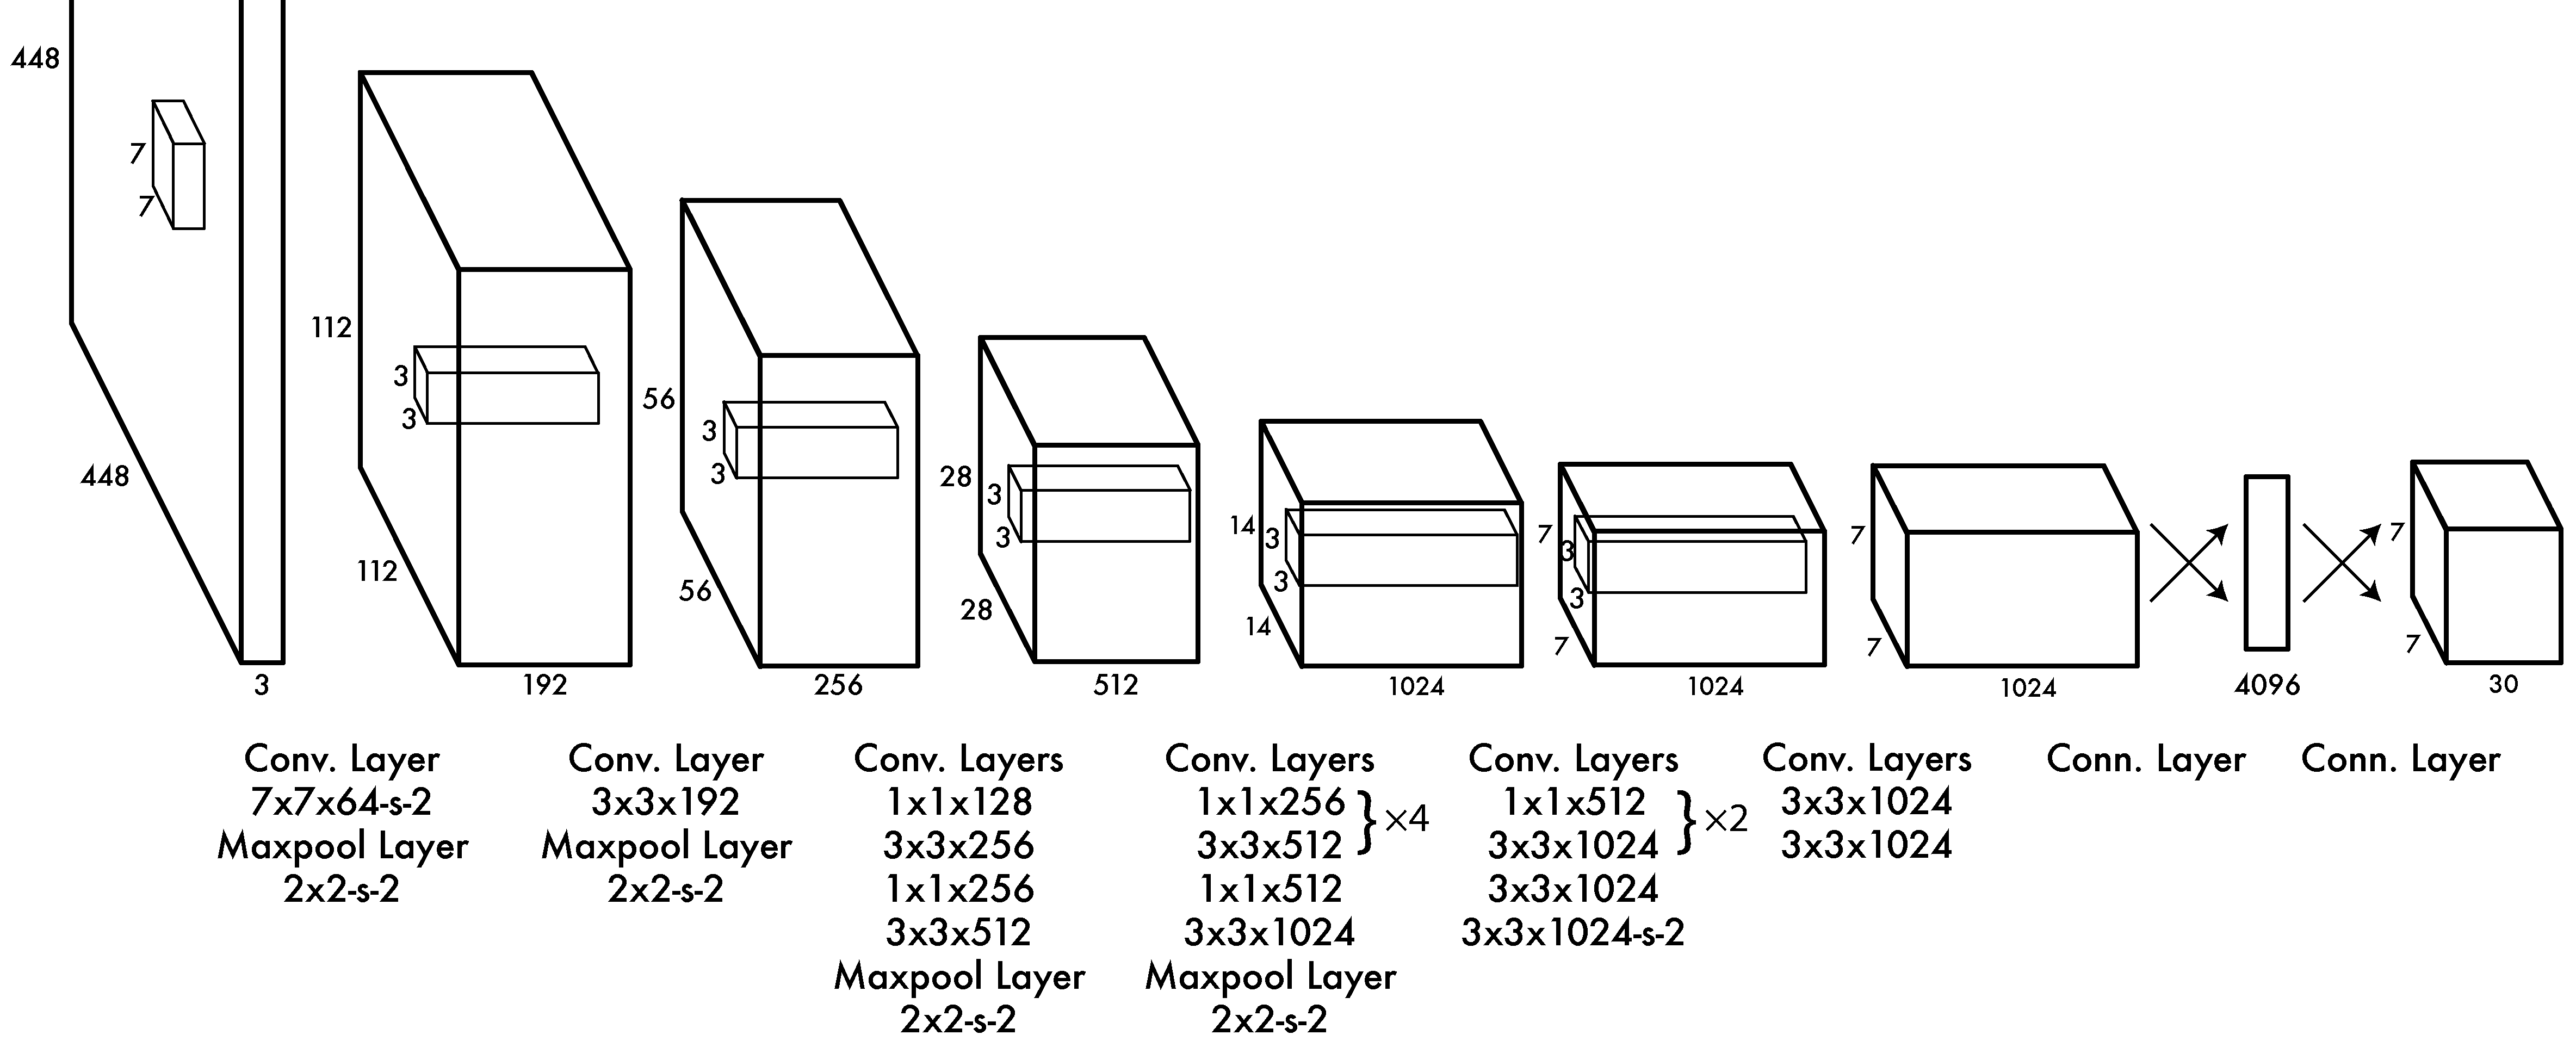
\includegraphics[width=0.8\textwidth]{Figures/yolo}
    \caption{Architektura původní verze YOLO \cite{yolo}}
    \label{fig:yolo}
\end{figure}

Každý bounding box je reprezentován souřadnicemi středu a velikosti (šířka a
výška). Dohromady s informací o jistotě detekce bounding boxu (confidence
score) vrátí model $5$ informací o každém bounding boxu. Pro každé pole mřížky
pak určí společnou informaci o třídě všech objektu v daném poli. Pokud objekt
není detekován, třída indikuje pozadí a souřadnice bounding boxu jsou
ignorovány. Velikost výstupního vektoru je tedy $7 \times 7 \times (2 * 5 +
    C)$, kde $C$ je počet definovaných tříd - v původní verzi pouze 20.

Tento algoritmus, navržený v roce 2015 J. Redmonem at al., byl revolučně
rychlý, zároveň v porovnání s jinými real time detekčními algoritmy dosahoval i
slušné přesnosti. Nicméně byl velice citlivý na velikost objektu a přesnost
detekce, zejména u menších objektů, byla horší než u dvoufázových algoritmů.

Další verze algoritmu YOLO přinesly postupná vylepšení ve formě optimalizace
trénování a architektury. YOLOv2 \cite{yolo9000} zavedl mj. trénování na
několika měřítkách a byl natrénován s 9000 třídami (proto taky nazýván
YOLO9000). YOLOv3 \cite{yolov3} přinesl mj. detekci na několika měřítkách.
Postupně byla taky zvětšována mřížka a měnila se použita architektura CNN sítě
sloužící pro extrakci příznaků pro jednotlivá pole mřížky. Postupně taky byly
přidávány další funkce jako je segmentace, detekce pózy či sledování objektů
(ang. tracking).

V 2020 roce firma Ultralytics poprve implementovala YOLO s využitím populární
knihovny PyTorch (YOLOv5), což umožnilo snadnější využití YOLO v praxi. Firma
Ultralytics taky vytvořila framework pro použití různých verzí YOLO (YOLOv3 a
novější). Taky pracuje na dalších vylepšeních a optimalizacích. Konkrétně
vytvořila YOLOv5 (2020), YOLOv8 (2023) a YOLOv11 (2024). Algoritmus YOLO je tak
mimo svoji rychlost a přesnost velice oblíbený právě kvůli jednoduchosti
použití, široké škále dostupných funkcí a kontinuálnímu vývoji.

\subsubsection{SSD}
Dalším populárním algoritmem, který používá jednofázový přístup, je SSD (z ang.
single shot detector). \cite{szegedy:ssd} Ten rozdělí vstupní obraz do několika
mřížek o různé velikosti. Postup je takový, že nejprve projde obraz konvoluční
síti, konkrétně síti VGG16, která extrahuje mapu příznaků. Tu se postupně
dalšími konvolučními vrstvami zmenšuje, výstup každého stádia zmenšení,
reprezentující mřížku dané velikosti, se spolu s původní mapou dále zpracovává
plně propojenou síti.
\begin{figure}[]
    \centering
    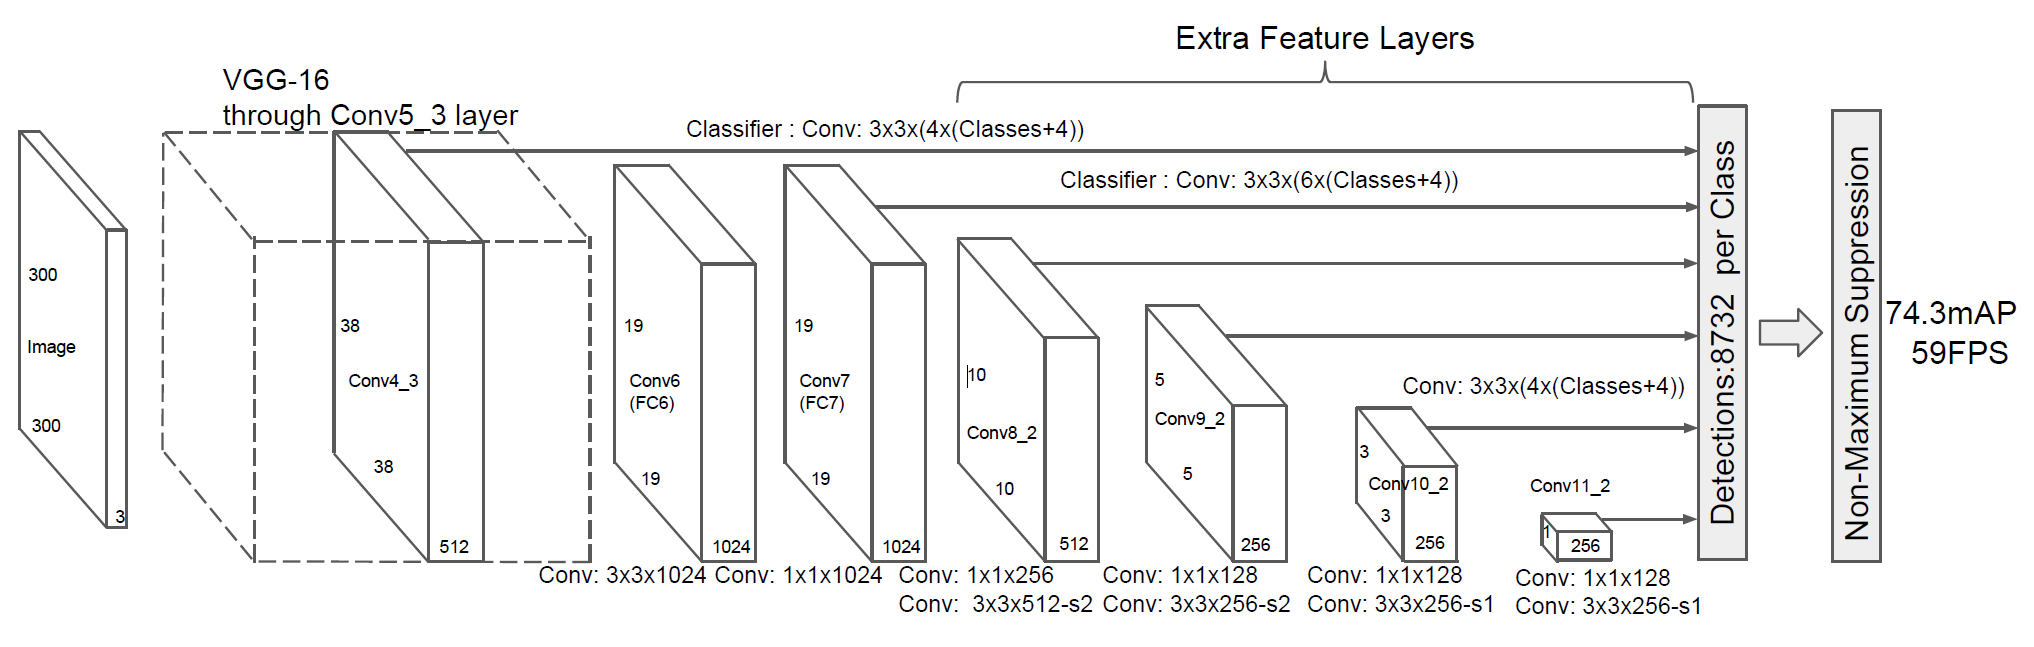
\includegraphics[width=0.8\textwidth]{Figures/ssd.png}
    \caption{Architektura SSD \cite{szegedy:ssd}}
    \label{fig:ssd}
\end{figure}

Výstupní bounding boxy nejsou, jako v případě YOLO, pouze výsledkem regrese,
ale pro každé pole dané mřížky je definováno několik výchozích oblastí (ang.
default box), ze kterých jsou vybrány ty, které obsahují objekt. K ním je
predikována třída objektu a posun i změna velikosti výchozí oblasti,
upřesňující výsledný bounding box.

V době svého vzniku byl SSD rychlejší a přesnější než YOLO, ale novější verze
YOLO jej už předběhly. Nicméně některé principy SSD, jako výchozí oblasti či
použití různých měřítek, byly převzaty do novějších verzí YOLO.

% openpifpaf, mediapipe(shufflenet, resnet), torchvision, yolo

\endinput